%%%%%%%%%%%%%%%%%%%%%%%%%%%%%%%%%%%%%%%%%
% Beamer Presentation
% LaTeX Template
% Version 1.0 (10/11/12)
%
% This template has been downloaded from:
% http://www.LaTeXTemplates.com
%
% License:
% CC BY-NC-SA 3.0 (http://creativecommons.org/licenses/by-nc-sa/3.0/)
%
%%%%%%%%%%%%%%%%%%%%%%%%%%%%%%%%%%%%%%%%%

%----------------------------------------------------------------------------------------
%	PACKAGES AND THEMES
%----------------------------------------------------------------------------------------

\documentclass{beamer}

\mode<presentation> {

% The Beamer class comes with a number of default slide themes
% which change the colors and layouts of slides. Below this is a list
% of all the themes, uncomment each in turn to see what they look like.

%\usetheme{default}
%\usetheme{AnnArbor}
%\usetheme{Antibes}
%\usetheme{Bergen}
%\usetheme{Berkeley}
%\usetheme{Berlin}
%\usetheme{Boadilla}
\usetheme{CambridgeUS}
%\usetheme{Copenhagen}
%\usetheme{Darmstadt}
%\usetheme{Dresden}
%\usetheme{Frankfurt}
%\usetheme{Goettingen}
%\usetheme{Hannover}
%\usetheme{Ilmenau}
%\usetheme{JuanLesPins}
%\usetheme{Luebeck}
%\usetheme{Madrid}
%\usetheme{Malmoe}
%\usetheme{Marburg}
%\usetheme{Montpellier}
%\usetheme{PaloAlto}
%\usetheme{Pittsburgh}
%\usetheme{Rochester}
%\usetheme{Singapore}
%\usetheme{Szeged}
%\usetheme{Warsaw}

% As well as themes, the Beamer class has a number of color themes
% for any slide theme. Uncomment each of these in turn to see how it
% changes the colors of your current slide theme.

%\usecolortheme{albatross}
%\usecolortheme{beaver}
%\usecolortheme{beetle}
%\usecolortheme{crane}
%\usecolortheme{dolphin}
%\usecolortheme{dove}
%\usecolortheme{fly}
%\usecolortheme{lily}
%\usecolortheme{orchid}
%\usecolortheme{rose}
%\usecolortheme{seagull}
%\usecolortheme{seahorse}
%\usecolortheme{whale}
%\usecolortheme{wolverine}


%\setbeamertemplate{footline} % To remove the footer line in all slides uncomment this line
%\setbeamertemplate{footline}[page number] % To replace the footer line in all slides with a simple slide count uncomment this line

%\setbeamertemplate{navigation symbols}{} % To remove the navigation symbols from the bottom of all slides uncomment this line
}
\usepackage[utf8]{inputenc}
\usepackage{amsmath}
\usepackage{graphicx} % Allows including images
\usepackage{booktabs} % Allows the use of \toprule, \midrule and \bottomrule in tables

%----------------------------------------------------------------------------------------
%	TITLE PAGE
%----------------------------------------------------------------------------------------

\title[Planck Stars]{Introduction to Plack Stars} % The short title appears at the bottom of every slide, the full title is only on the title page

\author[Hernández A.]{Alejandro Hernández A. } % Your name
\institute[Uniandes] % Your institution as it will appear on the bottom of every slide, may be shorthand to save space
{
Universidad de los Andes, Bogotá, Colombia \\ % Your institution for the title page
%\medskip
%\textit{a.hernandez105@uniandes.edu.co}\\
%\textit{jd.prada1760@uniandes.edu.co}
 % Your email address
}
\date{November 6, 2015} % Date, can be changed to a custom date

\begin{document}

\begin{frame}
\titlepage % Print the title page as the first slide
\end{frame}

\begin{frame}
\frametitle{Overwiew} % Table of contents slide, comment this block out to remove it
\tableofcontents % Throughout your presentation, if you choose to use \section{} and \subsection{} commands, these will automatically be printed on this slide as an overview of your presentation
\end{frame}

%----------------------------------------------------------------------------------------
%	PRESENTATION SLIDES
%----------------------------------------------------------------------------------------

%------------------------------------------------
\section{Introduction} % Sections can be created in order to organize your presentation into discrete blocks, all sections and subsections are automatically printed in the table of contents as an overview of the talk

\begin{frame}
\frametitle{Introduction}

\textbf{Einstein Field Equations} \\\

\begin{equation}
\label{field}
R_{\mu \nu} - \frac{1}{2} R g_{\mu \nu} + \Lambda g_{\mu \nu} = 8 \pi T_{\mu \nu}
\end{equation}

\
\\
\
\\

\textbf{Minkowski metric} \\\

\begin{equation}
\label{mink}
ds^2 = -dt^2 + dr^2 + r^2d\Omega ^2
\end{equation}


\end{frame}

%------------------------------------------------

%\subsection{Introduction} % A subsection can be created just before a set of slides with a common theme to further break down your presentation into chunks

\subsection{Black hole solutions}

\begin{frame}
\frametitle{Black hole solutions}

\textbf{Classification of Black holes}\\\
\\\


\begin{center}
  \begin{tabular}{| c | c | c |}
    \hline
     & Non-rotating ($J=0$) & Rotating ($J\neq 0$)\\ \hline
    Uncharged ($Q =0 $) & Schwarzschild & Kerr \\ \hline
    Charged ($Q \neq 0$) & Reissner-Nordstr\"om & Kerr-Newman \\
    \hline
  \end{tabular}
\end{center}
\end{frame}


\section{Regularized Schwarzschild metric}
%OJO Explicar que solo se aborda la parte estática en las tres instancias de formación del agujero negro
\begin{frame} % Need to use the fragile option when verbatim is used in the slide
\frametitle{Schwarzschild Black hole}

\textbf{Schwarzschild metric}
\begin{equation}
\label{sch}
ds^2 = -\left(1 - \frac{2m}{r} \right) dt^2 + \left(1 - \frac{2m}{r} \right)^{-1}dr^2 + r^2d\Omega ^2
\end{equation}

\
\\
\
\\

\textbf{Kretschmann invariant}
\begin{equation}
\label{kret}
\kappa = R^{\alpha \beta \gamma \delta} R_{\alpha \beta \gamma \delta} = \frac{48m^2}{r^6}
\end{equation}
\end{frame}

%------------------------------------------------

\begin{frame}
\frametitle{Regularized Schwarzschild metric}
According to \cite{hayward}, we cand find metrics that are:

\begin{itemize}
\item Spherically symmetric.
\item Static.
\item Asymptotically flat (minkowski).
\item \textbf{Have regular center.}
\end{itemize}

The resulting stress-energy tensor is physically reasonable, satisfies the weak energy condition and has components that are bounded and fall off appropriately at large distance.

%OJO Condiciones de energía, y el comentario de horizontes de Cauchy.

\end{frame}

\begin{frame}
\frametitle{Energy conditions}
\textbf{Null energy condition}\\
For every null vector $x$:\ \ \ \ \ \ \ \ \ $T_{\mu \nu}x^{\mu}x^{\nu} \geq 0$.\\\ 

\textbf{Weak energy condition}\\
For every timelike vector $x$:\ \ \ \ $T_{\mu \nu}x^{\mu}x^{\nu} \geq 0$.\\\

\textbf{Dominant energy condition}\\
For every timelike vector $x$:\ \ \ \ $T_{\mu \nu}x^{\mu}x^{\nu} \geq 0$, \ \ \ \ $T_{\mu \nu}T^{\nu}_{\lambda}x^{\mu}x^{\lambda} \leq 0$.\\\

\textbf{Strong energy condition}\\
For every timelike vector $x$:\ \ \ \ $T_{\mu \nu}x^{\mu}x^{\nu} \geq \frac{1}{2}T^{\lambda}_{\lambda}x^{\sigma}x_{\sigma}
$. 

\end{frame}

%------------------------------------------------



%------------------------------------------------

\begin{frame}
\frametitle{Regularized Schwarchild metric}
Consider a static, spherically symmetric metric of the form:

\begin{equation}
ds^2 = -F(r)dt^2 + \frac{1}{F(r)}dr^2 + r^2d\Omega ^2
\end{equation}

We demand

\begin{equation}
F(r) \sim 1 - \frac{2m}{r}\ \ \ as\ \ \ r \rightarrow \infty
\end{equation}

\begin{equation}
F(r) \sim 1 - \frac{r^2}{l^2}\ \ \ as\ \ \ r \rightarrow 0
\end{equation}

%OJO - l densidad de energía y hubble length.

\end{frame}

\subsection{Hayward metric}

\begin{frame}
\frametitle{Hayward metric}
The so called Hayward metric \cite{hayward} satisfies all the required properties and is given by:

\begin{equation}
F(r) = 1 - \frac{2mr^2}{r^3 + 2ml^2}
\end{equation}

where $l$ encodes the central energy density $\frac{3}{8\pi l^2}$. Therefore

\begin{equation}
ds^2 = -\left( 1 - \frac{2mr^2}{r^3 + 2ml^2} \right)dt^2 + \frac{1}{\left( 1 - \frac{2mr^2}{r^3 + 2ml^2} \right)}dr^2 + r^2d\Omega ^2
\end{equation}

\end{frame}


\begin{frame}
\frametitle{Hayward metric}

Analyzing the zeros of $F(r)$, we get a critical mass $m_{*} = \frac{3\sqrt{3}}{4}l$ and a radius $r_{*} = \sqrt{3}l$.

\begin{itemize}
\item No zeros if $m < m_{*}$. ($\leftrightsquigarrow$ Regular space time with the same causal structure as a flat space-time).
\item One double zero at $r = r_{*}$ if $m = m_{*}$.
($\leftrightsquigarrow$ Regular extreme black hole with degenerate Killing horizon).
\item Two simple zeros at $r = r_{\pm}$ if $m > m_{*}$.
($\leftrightsquigarrow$ Regular nonextreme black hole with both outer and inner Killing horizons located at $r_{+} \approx 2m$ and $r_{-} \approx l$ for $m \gg m_{*}$). %OJO con el mass gap
\end{itemize}
\end{frame}

\begin{frame}
\begin{figure}[h!]
	\centering
	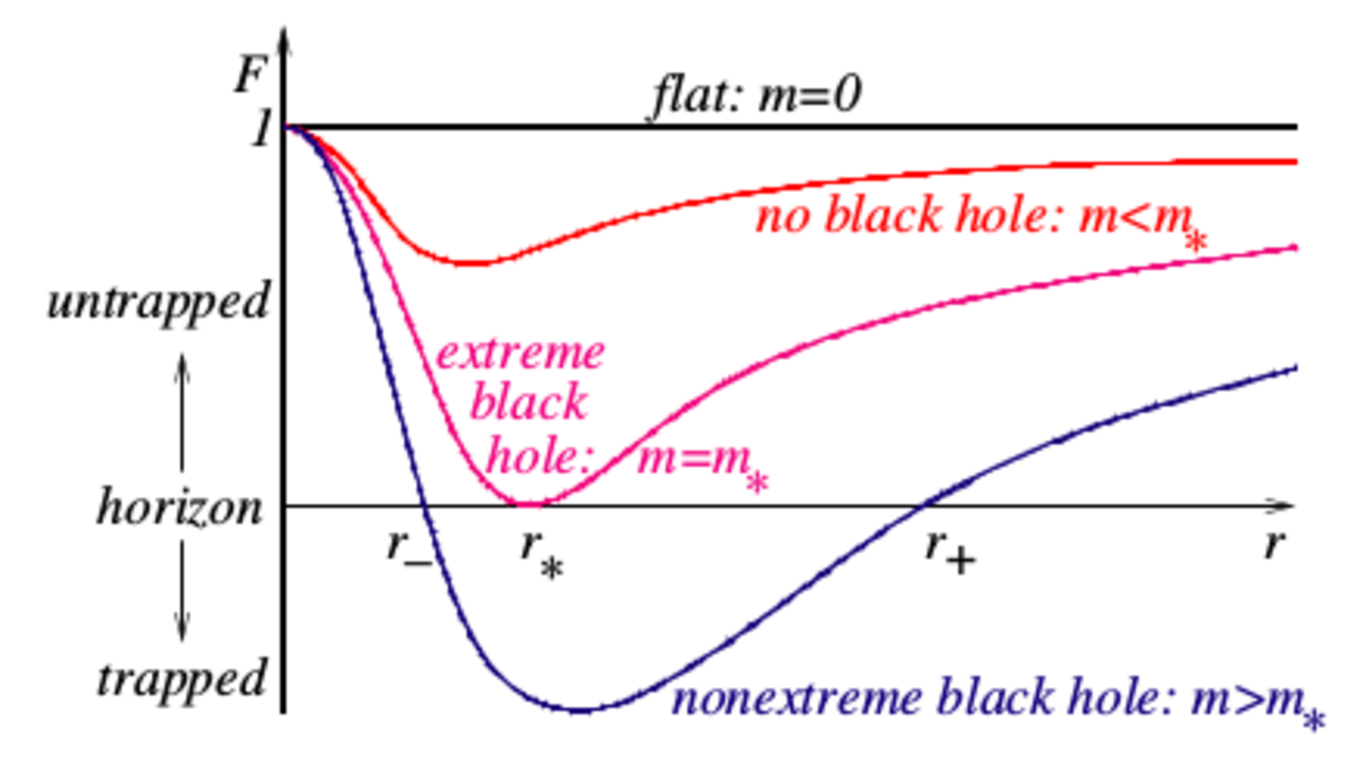
\includegraphics[width=0.7\textwidth]{F(r)}
	\caption{Behaviour\footnote{Image taken from \cite{hayward}.} of $g_{tt} = F(r)$ for different values of the parameter $m$.}
	
\end{figure}

\end{frame}

\begin{frame}
\frametitle{Hayward metric}
If we use field equations \ref{field}, we note that this metric is supported by density $-T^{t}_{t}$, radial pressure $T^{r}_{r}$, and transverse pressure $T^{\theta}_{\theta} = T^{\phi}_{\phi}$ given by:

\begin{equation}
G^{t}_{t} = G^{r}_{r} = - \frac{12l^2m^2}{\left( r^3 + 2l^2m \right)^2}
\end{equation}

\begin{equation}
G^{\theta}_{\theta} = G^{\phi}_{\phi} = \frac{24\left( r^3 - l^2m \right)l^2m^2}{\left( r^3 + 2l^2m \right)^3}
\end{equation}

They fall off very rapidly $\mathcal{O}(r^{-6})$.
% OJO As required for the components of a physically reasonable

%OJO Con la radiación
%
\end{frame}


\section{Quantum Field Theory}

\begin{frame}
\frametitle{Quantum Field Theory}
Spacetime metric describing 'non-singular' black holes are commonly studied in the literature \cite{effective,planck stars} as effective modification to the Schwarzschild solution that mimic quantum gravity effects removing the central singuarity.\\\

To begin with, two insights from quantum cosmology \cite{ashtekar}:

%OJO Especificar que al hablar de gravedad cuántica es realmente teoría cuántica de campos efectiva.
\begin{itemize}
\item The onset of quantum gravitational effects is when energy density reaches the Plank scale ($\sim 5.155 \cdot 10^{96}\ \frac{kg}{m^3}$).\\\

\item The dominant quantum effect at high density is a strong pressure, sufficient to counterbalance weight and reverse gravitational collapse.
\end{itemize} 
\end{frame}

\begin{frame}
\frametitle{Plack scale}

Planck scale is given by\\\	
\begin{center}
	\begin{tabular}{| c | c |}
    \hline
    \textbf{Quantity} & \textbf{SI equivalent} \\ \hline
    Planck time & $t_{p} = 5.39121 \cdot 10^{-44} s$\\ \hline
    Planck mass & $m_{p} = 2.17645 \cdot 10^{-8} kg$\\ \hline
    Planck length & $l_{p} = 1.616252 \cdot 10^{-35} m$\\ \hline
    \end{tabular}
\end{center}
\
\\
\
\\

and the Plack density is the quotient

\begin{equation}
\rho _{p} = \frac{m_{p}}{l_{p}^3} \approx 5.155 \cdot 10^{96}\ \frac{kg}{m^3}
\end{equation}
\end{frame}

\begin{frame}
\frametitle{Quantum Field theory}

For a black hole, the previous arguments imply that matter's collapse can be stopped before the central singularity is formed, yielding the formation of a central core, called a \textbf{Planck star} \cite{planck stars}.\\\

Nevertheless, several metrics describing non-singular black holes possess two unphysical characteristics:

\begin{itemize}
\item A clock in the regular center is not delayed with respect to a clock at infinity \cite{planck stars}.\\\
%OJO explicar el por qué de esto. Centrarse en lo de F(r) = 1

\item They do not reproduce the corrections to Newton potential derived from an effective treatment of quantum gravitational theory \cite{bohr}.
\end{itemize}

%OJO En otras palabras, podemos definir una estrella de Plack
\end{frame}


\subsection{Newton Potential}

\begin{frame}
\frametitle{Newton potential}

The quantum corrections to the Newton potential can be obtained using effective field theory \cite{bohr}, and reintroducing the Planck length, they are given by:

\begin{equation}
\Phi (r) = -\frac{m}{r} \left( 1 + \beta \frac{l_{p}^2}{r^2}\right) + \mathcal{O}(r^4)
\end{equation}

Since

\begin{equation}
\Phi (r) = -\frac{1}{2} \left( 1 + g_{tt} \right)
\end{equation}

\begin{equation}
g_{tt} = - F(r) = -1 + \frac{2m}{r} - \frac{4l^2m^2}{r^4} + \mathcal{O}(r^{-5})
\end{equation}

We require additional adjustments to the Hayward metric.

\end{frame}

\subsection{Modified Hayward metric}

\begin{frame}
\frametitle{Modified Hayward metric}
The most general spherically symmetric, static metric that includes the previously mentioned corrections is \cite{effective}:

\begin{equation}
ds^2 = -G(r)F(r)dt^2 + \frac{1}{F(r)}dr^2 + r^2d\Omega^2
\end{equation}

The physical requirements imposed on $G(r)$ are:

\begin{itemize}
\item Preserve the Schwarzschild behaviour at large $r$.
\item \textbf{Include the quantum corrections of the Newton potential.}
\item Allow a final time dilatation between $r = 0$ and $r \rightarrow \infty$.
\item Near the center, the metric is still de Sitter.	
\end{itemize}

In particular, we can take

\begin{equation}
G(r) = 1 - \frac{\beta m \alpha}{\alpha r^3 + \beta m}
\end{equation}

\end{frame}

\section{Conclusions}

\begin{frame}
\frametitle{Conclusions}
\small
\begin{itemize}
\item Spacetime singularities are unavoidable in gravitational collapse, if the classical theory of general relativity is valid at all scales and the stress-energy tensor of matter satisfies the classical energy conditions.\\\

\item General relativity cannot be valid at all scales because of quantum mechanics.\\\

\item There is a certain expectation that near the center of a physical black hole quantum effects dominate, and prevent the formation of the singularity.\\\

\item Planck stars are one possible way to include effective QFT correction in general relativity.\\\

\item Hayward metric by itself does not cover all the desirable quantum correction into the Schwarzchild metric, therefore the proposal of a modified Hayward metric.

\end{itemize}
\end{frame}

\section{References}

\begin{frame}
\frametitle{References}
\footnotesize{
\begin{thebibliography}{99} % Beamer does not support BibTeX so references must be inserted manually as below

\bibitem[Hayward, 2006]{hayward} Hayward, S.A.: Formation and Evaporation of regular black holes. Phys. Rev. Lett. \textbf{96}, 31103 (2006).

\bibitem[De Lorenzo, 2015]{effective} De Lorenzo, T., Pacilio, C., Rovelli, C., Speziale, S.: On the effective metric of a Planck star. Gen. Relativ. Gravit. \textbf{47}, 41 (2015).

\bibitem[Mazur, 2001]{mazur} Mazur, P. O., Mottola, E.: Gravitational condensate stars: An alternative to black holes, arXiv:gr-qc/0109035 

\bibitem[Ashtekar, 2007]{ashtekar} Ashtekar, A., Pawlowski, T., Singh, P., Vandersloot, K.: Loop quantum cosmology of k=1 FRW models. Phys. Rev. D \textbf{75},24035 (2007).

\bibitem[Rovelli, 2014]{planck stars} Rovelli, C., Vidotto, F.: Planck Stars. Int. J. Mod. Phys. D. \textbf{23}, 1142026, (2014).

\bibitem[Bjerrum-Bohr,2003]{bohr} Bjerrum-Bohr, N.E.J., Donoghue, J.F., Holstein, B.R.: Quantum gravitational corrections to the non-relativistic scattering potential of two masses. Phys. Rev. D \textbf{67}, 084033 (2003). 



\end{thebibliography}
}
\
\end{frame}



\begin{frame}
\Huge{\centerline{The End}}
\end{frame}

%----------------------------------------------------------------------------------------

\end{document} 